\section{Crossing comparisons along the random trajectory}
\label{sec:crossings}

The trajectory of Theorem~\ref{traj:critical-trajectory} has
$X_k\to0$, but its decay need not be summable.  We prove that every fixed
finite collection of macroscopic crossing and passage tests nevertheless
has asymptotically the same law as in the pure model.  The gain comes
from the size of the square
changed at one step: small squares can affect a macroscopic test only
when several contour passages reach far beyond that square.  We first
establish uniform conditional bounds for those passages, keeping the
marks of each reversal separate throughout the argument.

\subsection{Geometric tests and the deterministic inputs}

Use the triangulation obtained by drawing the northwest--southeast
diagonal in every lattice square, and interpolate the spins affinely.
Its zero contours implement the prescribed north--east,
south--west resolution up to a matched displacement of order one lattice
spacing.  A colored path uses vertices of one spin sign and edges of this
triangulation.  A polygonal corridor is a closed topological rectangle
with two opposite boundary arcs designated as gates; its crossing test
asks for a colored path between the gates.  A polygonal band is the
region between two disjoint simple polygons; its circuit test asks for a
colored path separating its boundary components.  We approximate these
sets by subcomplexes of the triangulation, preserving the cyclic order
of their marked sides, with error of order one lattice spacing.  The
polygons are fixed and nondegenerate, and every test has a specified open
neighborhood in which spins remain free.

A contour passage between two terminal sets is a contour subarc joining
them whose interior lies in the prescribed permitted region.  Different
passages have disjoint open parameter intervals on each contour; their
endpoints may coincide at terminal hits.  Thus repeated passages of one
contour are counted separately.  Cropping at the last visit to the first
terminal before the first visit to the second gives this convention.
It is the passage convention of \cite[Section~5, ``Tests, passages, and
independent marks'']{S}.

For a center $z$, direction $\alpha$, and $0<r<R$, put
\[
 S_r(z,\alpha)=z+e^{i\alpha}[-r,r]^2,
 \qquad A(z,\alpha;r,R)=S_R(z,\alpha)\setminus\operatorname{int}S_r(z,\alpha).
\]
We use three checks:
\begin{align}
 F_4(z,\alpha;r,R)&=\{\text{at least four passages across }A(z,\alpha;r,R)\},
 \nonumber\\
 H_2(z,\alpha;r,R)&=\{\text{at least two such passages confined to }
 z+e^{i\alpha}\{\operatorname{Im}w\geq0\}\},
 \label{cross:checks}\\
 F_1(z,\alpha;r,R)&=\{\text{at least one passage across }A(z,\alpha;r,R)\}.
 \nonumber
\end{align}
The straight line in $H_2$ is a confinement wall inside a bulk chart;
no spins are pinned on that line.  Its terminals are the inner and outer
square boundaries.  Fixed proportional crops, and fixed unions covering
the two possible half-planes, will be included whenever the geometry
requires them.

Here are the deterministic inputs from the companion, with
their order of limits.  For pure critical spins in buffered bulk charts,
\begin{equation}
 \begin{aligned}
 \limsup_{\delta\downarrow0}\Prob_0(F_4(r,R))
 &\leq C(r/R)^{2+c_0},&
 \limsup_{\delta\downarrow0}\Prob_0(F_1(r,R))
 &\leq C(r/R)^{c_0},\\
 \limsup_{\delta\downarrow0}\Prob_0(H_2(r,R))&=o(r/R).
 \end{aligned}
 \label{cross:pure-input}
\end{equation}
Here $c_0>0$, and the ratio is fixed before the mesh limit.  These are
\cite[Section~2, Propositions ``Iterated four-passage bound'' and ``Pure
buffered RSW consequences''; Section~5, Proposition ``Two bulk passages
confined to a half-plane'']{S}.  The conditional density comparison in
\cite[Section~2, Corollary ``Two collars around an annulus'']{S}
bounds the law on an annular support under arbitrary pins outside fixed
proportional inner and outer collars by $D$ times its pure bulk marginal.
The constant $D$ does not grow with the annulus ratio.  These inputs also
allow translations, rotations, and the fixed crops just specified.

Choose a fixed gap factor $G$ large enough to separate the collars in
successive rings.  Fix in advance smaller proportional collars that will
survive the boundary erosions below.  Include in $D$ the comparison
constant for those collars and the finite losses for crops and
half-plane choices, then choose a large fixed ratio $a$.  The bounds in
\eqref{cross:pure-input} give exponents and positive tolerances satisfying
\begin{equation}
 p_4>2,\qquad p_h>1,\qquad p_1>0,
 \qquad q_i^0+\tau_i<(Ga)^{-p_i}\quad(i=4,h,1),
 \label{cross:slack}
\end{equation}
where $q_i^0$ already includes the conditional density loss.
For the middle inequality, first use $o(a^{-1})$ to obtain strict slack
below $(Ga)^{-1}$, and only then choose $p_h>1$ sufficiently close to one.
No specified half-plane power law is required.  Increase the starting
scale so that the same $q_i^0$ bounds hold at finite mesh for all three
fixed shapes of ratio $a$.  Uniformity in the frame follows by compactness
of directions and normalized offsets, using slightly relaxed radii.
All these choices precede the choice of the weak-randomness interval.

We also use the following purely geometric implication from
\cite[Section~5, Lemma ``Passages forced by a pivotal square'']{S}.
For a corridor crossing, band circuit, or one of the three checks $T$,
there is a positive geometry scale $a_T$
such that a change confined to a square of radius $b<a_T$ about $z$
can change $T$ only if its common exterior contours supply four passages
between scales $b$ and $u$, two half-plane passages between $u$ and $v$,
and one passage between $v$ and $a_T$, where
\begin{equation}
 u=\min\{a_T,\max\{b,\dist(z,\mathcal E_T)\}\},\qquad
 v=\min\{a_T,\max\{b,\dist(z,\mathcal V_T)\}\}.
 \label{cross:distances}
\end{equation}
Here $\mathcal E_T$ and $\mathcal V_T$ are the unions of the sides and
vertices of its polygons.  In particular $b\leq u\leq v\leq a_T$.
The scale $a_T$ is smaller than every relevant side length, terminal
separation, and separation of nonincident sides.  A fixed number of
rings may be omitted near transitions; half-plane rings may be
recentered on a side and the last rings near a vertex.  For each of the
three check shapes, $a_T$ is a fixed small multiple of its inner radius
$r$.  We choose that multiple small enough that every retained ring has
inner radius at most $r/2$ and its collars remain in the prescribed free
neighborhood.  This implication concerns arbitrary fillings of the
changed square and therefore also applies to a square whose values may
be chosen after other edits.


\begin{figure}[tb]
 \centering
 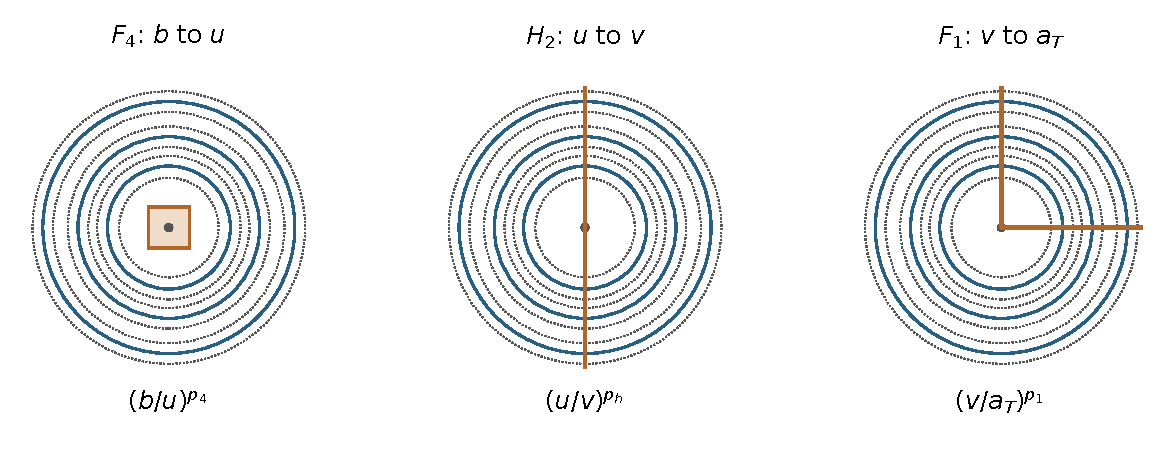
\includegraphics[width=\textwidth]{figures/pivotal-rings.pdf}
 \caption{The three ranges of checks forced by a pivotal square,
 schematically.  Blue rings have separated dotted collars; their centers
 may change between ranges.  Orange denotes the edit square, a side,
 and a vertex of the test, respectively, rather than a domain boundary.
 The drawing suppresses the actual contour passages and does not depict
 the literal gap ratios.  Enlarged environment neighborhoods fit in
 these separated collars, and the first retained ring avoids the
 environment stencil of the inserted mark.}
 \label{cross:fig-rings}
\end{figure}

\subsection{Conditional specifications and one reversal}

In the remainder of the proof lengths are lattice lengths unless a
factor $\delta$ is displayed.  Write $\eta$ for the full environment,
including the independent priorities and thresholds used to construct
the potentials.  A Gibbs variable includes both spins and reference
auxiliary variables, and is denoted by $\chi$.  At level $k$, in a finite
free chart $W$, with exterior configuration $\zeta$, the specification is
\begin{equation}
 \mu_{k,\eta,W}^{\zeta}(\dd\chi_W)
 =\frac{\exp F_{k,W}^{\zeta}(\chi_W)}
 {\mu_{0,W}^{\zeta}(\exp F_{k,W}^{\zeta})}
 \mu_{0,W}^{\zeta}(\dd\chi_W),\qquad
 F_{k,W}^{\zeta}=\sum_{j:\,\supp f_j^{(k)}\cap W\ne\varnothing}
 f_j^{(k)}(\chi_W\zeta_{W^c}).
 \label{cross:specification}
\end{equation}
The reference specification is pure critical Ising times its independent
reference auxiliary variables.  We may condition again in a smaller
free chart.  All suprema below include every exterior spin and auxiliary
assignment, so they also bound conditional laws with a random exterior.

Corollary~\ref{map:locality} allows the local construction to be performed
inside a free chart.  The prescribed exterior $\zeta$ contains only
level-$k$ field variables.  If a parent's complete decoration and
allocation stencil leaves $W$, set its $F_j$ to zero in every new coin
likelihood and retain its child logs.  Keep the full comparison stars
and the usual dummy coins.  Every fresh coin with a nontrivial
decoration is then sampled inside $W$.  Perform integrations only when
their full stencils lie in $W$.  Frozen terms, including terms entering
from outside $W$, are included in any
integration they meet; the exclusion rule still prevents a term from
meeting two integration squares.  Skip special integrations near the
boundary by the same rule.  The resulting identity is exact, and its
conditional specification agrees with the full level-$(k+1)$
specification at distance at least $C_1s_{k+1}$ from the boundary.
Only after constructing this joint output law do we condition outside
the eroded interior, whose exterior may now include fresh coins.
Disintegration gives a mixture of level-$(k+1)$ conditional
specifications; each is bounded by the corresponding exterior supremum.  This argument uses local conditional
identities, and does not condition on a favorable boundary event.

For a check on $A(z,\alpha;r,ar)$ take the surrounding chart
$W=S_{2ar}(z,\alpha)\setminus S_{r/2}(z,\alpha)$.  To iterate the
local construction in this fixed chart, allow the
available chart at level $k$ to be
$W_k=W\ominus M_1s_k$, where $\ominus t$ removes points within distance
$t$ of its boundary.  Choose $M_1$ so that
$M_1s_{k+1}\geq M_1s_k+C_1s_{k+1}$; it may also absorb allocated-support
overhangs.  Choose $M_0$ much larger than $M_1$ and all stencil constants.
Then a check with inner radius $r\geq M_0s_k$ retains the smaller
proportional collars chosen above in $W_k$, and successive interior steps
retain them as long as the check is still in this range.  Raise the first
retained radius, if necessary, so that the already fixed
ring gaps separate all environment stencils as well as the free charts.
The factor $G$ and the slack in \eqref{cross:slack} remain fixed.

By Proposition~\ref{map:reversal}, reversing step $k$ can change spins only in
squares of radius
\begin{equation}
 b_k=5s_{k+1},\qquad
 \E p_{x,k}(\eta)\leq C_LX_k,
 \label{cross:mark-bound}
\end{equation}
centered on the parent grid; increasing the fixed factor five absorbs
rounding if necessary.  Conditional on $\eta$, these Bernoulli marks
are mutually independent and independent of the entire new Gibbs
sample, including its fresh coins, before any further conditioning.
Their parameters depend only on environment variables within a fixed
multiple of $s_{k+1}$ of the center.  They can be placed at every candidate
center, independently of which integrations were selected.  The same
upper parameter envelope works for the localized construction.

For clarity, the elementary reason for this domination is a lower
likelihood-ratio bound.  If $S_x$ is a fixed constant times the sum of
child norms in the update stencil, then, conditional on the fresh coins
and the common exterior of the integration squares, the
before-integration law has density at least $e^{-S_x}$ relative to the
after-integration law.  It is therefore a
mixture with weight $e^{-S_x}$ of the new law and a residual probability
law.  On a Bernoulli mark of parameter $1-e^{-S_x}$ use the residual law;
otherwise retain the new sample.  Uniformly in all boundary data,
$1-e^{-S_x}\leq\min\{1,S_x\}$, which gives
\eqref{cross:mark-bound}.  Conditional separation of the update squares
permits independent marks, including for the special ratio integrations.
Integrating the discarded fresh coins out of the reconstructed decorated
law recovers the old spin law with its originally prescribed
level-$k$ exterior.

Given a spin configuration $\sigma$ and marks $M$ from just one reversal,
let $\mathcal C(\sigma,M)$ be the configurations agreeing with $\sigma$
off the marked squares.  For a Boolean test $T$, put
\begin{equation}
 \begin{aligned}
 T^+(\sigma,M)&=\1\{T(\widetilde\sigma)=1
       \text{ for some }\widetilde\sigma\in\mathcal C(\sigma,M)\},\\
 D_T(\sigma,M)&=\1\{T\text{ is not constant on }\mathcal C(\sigma,M)\}.
 \end{aligned}
 \label{cross:possibility}
\end{equation}
Both are increasing in the marks, irrespective of spin monotonicity.
For a check $T$ of inner radius $r$ in its prescribed annular chart, define
\begin{align}
 B_{k,T}(\eta)&=\sup_\zeta\mu_{k,\eta,W_k}^{\zeta}(T),\nonumber\\
 B^+_{k,T}(\eta)&=\sup_\zeta
  (\mu_{k,\eta,W_k}^{\zeta}\otimes\pi_{k-1,\eta})(T^+),
 \label{cross:envelopes}
\end{align}
where $\pi_{k-1,\eta}$ is the independent mark law for reversal of step
$k-1$.  At $k=0$ only the plain bound is used.  The supremum is taken
before environmental expectation.  Only finitely many exterior field
variables can enter these finite charts;
the auxiliary variables have finite alphabets, so these suprema are
measurable finite maxima.  Each quantity is a function only of
the environment in the chart and a fixed $O(s_k)$ neighborhood: these
are the supports of the potentials touching the chart and of the mark
parameters whose squares meet the test.  Mixtures over exterior data
need not have this locality; the suprema do.

\subsection{The product bound and the location count}

The next lemma supplies the single-step error.  Its hypothesis will be
proved by induction, first for the three fixed check shapes, and then
used for any prescribed polygonal test.

\begin{lemma}[A single-level pivotal bound]
\label{cross:single-level}
Let spins have the level-$k$ specification in a free chart, and allow
marks from step $k-1$, of radius $b=5s_k$.  Suppose the possibility envelope for every retained ring check satisfies
$\E B^+_{k,T_i}\leq q_i^0+\tau_i$.  The rings start at a sufficiently
large fixed multiple of $b$ and have disjoint collars enlarged by all
spin, mark, and environment stencils.  Then the expected conditional
supremum of the probability that a fixed test $T$ is changed by these
marks is at most
\begin{equation}
 C_TX_{k-1}\min\{1,(s_k/a_T)^c\},
 \label{cross:one-step-error}
\end{equation}
for a fixed $c>0$.  The same bound controls the increase from $T$ to
$T^+$.  Constants are uniform over translates, rotations, and dilates of
each of the three check shapes.  Any deterministic partial activation
of the marks satisfies the same estimates.
\end{lemma}

\begin{proof}
Activate the finitely many relevant marks in deterministic order.
For fixed $\eta$ and exterior data, conditioning on all previous marks
charges the first instability at $x$ to
$p_{x,k-1}(\eta)$ times a pivotal possibility event with that mark omitted.
If adding its square first permits two test values, choose a witnessing
assignment and revert the new square, retaining all the other assigned
values.  The resulting pair differs only in that square.  Every passage
required outside it by the geometric implication is consequently
possible using only the previous marks.  We may enlarge these to all
other marks in their respective ring neighborhoods.

Consider a retained family of rings with checks $T_1,\ldots,T_m$.
For fixed environment, condition off the first ring's eroded chart
$W_{1,k}$ and on the marks whose squares do not meet its spin support.  The other ring
checks are measurable under this conditioning; the remaining spins have
the specified conditional Gibbs law, and the remaining marks retain
their independent law.  Its factor is at most
$B^+_{k,T_1}(\eta)$.  Remove each ring in turn.  Pointwise in the original
exterior data this proves
\begin{equation}
 \sup_\zeta\bigl[p_{x,k-1}(\eta)
     \Prob_{k,\eta}^{\zeta}(T_1^+\cap\cdots\cap T_m^+)\bigr]
 \leq p_{x,k-1}(\eta)\prod_{\ell=1}^m B^+_{k,T_\ell}(\eta).
 \label{cross:quenched-product}
\end{equation}
The enlarged ring neighborhoods are disjoint and avoid the environment
stencil of $p_{x,k-1}$.  All factors on the right are therefore functions
of disjoint sets of the underlying independent environment variables.
Taking their expectation, including that of the inserted mark, gives
\begin{equation}
 \E\left[p_{x,k-1}\prod_{\ell=1}^m B^+_{k,T_\ell}\right]
 =\E p_{x,k-1}\prod_{\ell=1}^m\E B^+_{k,T_\ell}
 \leq C_LX_{k-1}\prod_{\ell=1}^m(q_{i(\ell)}^0+\tau_{i(\ell)}).
 \label{cross:annealed-product}
\end{equation}
This is why conditional exterior suprema, and the omission of rings
near the inserted square, are needed.  A product of unconditional
quenched check probabilities would not justify this equality.

Retain rings of ratio $a$ with successive inner radii in ratio $Ga$ in
each of the three ranges in \eqref{cross:distances}, illustrated in
Figure~\ref{cross:fig-rings}.  A fixed number of
omissions handles their endpoints, recenterings, and transitions.  By
\eqref{cross:slack}, the product in
\eqref{cross:annealed-product}, apart from $C_LX_{k-1}$, is at most
\begin{equation}
 C_T(b/u)^{p_4}(u/v)^{p_h}(v/a_T)^{p_1}.
 \label{cross:pivotal-power}
\end{equation}
If a range has too few scales for a retained ring, its bounded factor
loss is included in $C_T$.

It remains to sum over edit locations.  Normalize $a_T=1$ and suppose
$b<1$.  The centers with dyadically specified truncated distances $u,v$
occupy area at most $C_Tuv$: near a vertex, the portion of side at
distance $O(v)$ has length $O_T(v)$ and its $u$-neighborhood has that
area; away from vertices use the finite total side length.  The class
$u=v=1$ covers the remaining interior centers.  Since the center grid
has spacing comparable to $b$, enlarging each class by one grid cell
gives at most $C_Tuv/b^2$ centers.  Its contribution is bounded by
\begin{align}
 C_TX_{k-1}\frac{uv}{b^2}(b/u)^{p_4}(u/v)^{p_h}v^{p_1}
 &=C_TX_{k-1}(b/u)^{p_4-2}(u/v)^{p_h-1}v^{p_1}.
 \label{cross:area-sum}
\end{align}
Put $d=\min\{p_4-2,p_h-1,p_1\}>0$.
The three base ratios in the last expression have product $b$;
each dyadic class therefore contributes at most $C_TX_{k-1}b^d$.
There are $O_T((1+\log(1/b))^2)$ classes.  Absorb this factor into
$b^{d/2}$ and take $c=d/2$.  For $b\geq1$, only $O_T(1)$ grid centers
have squares meeting the test support, and the crude pivotal bound one
gives $C_TX_{k-1}$.  This proves \eqref{cross:one-step-error}, after
restoring $a_T$.  Finally $T^+-T\leq D_T$, and partial activation only
reduces the permitted mark parameters.
\end{proof}

\subsection{A bootstrap with geometrically weighted errors}

\begin{proposition}[Uniform conditional check bounds]
\label{cross:bootstrap}
Fix the preceding geometry and step constants.  There is $\varepsilon_*>0$
such that if the tuned trajectory satisfies $\sup_jX_j\leq\varepsilon_*$,
then, for every check $T_i$ of ratio $a$ and inner radius $r\geq M_0s_k$,
\begin{align}
 \E B_{k,T_i}
 &\leq q_i^0+C_{\rm boot}\sum_{j=k}^{J(r)}X_j(s_j/r)^c,
 \label{cross:plain-bootstrap}\\
 \E B^+_{k,T_i}
 &\leq q_i^0+C_{\rm boot}\sum_{j=k}^{J(r)}X_j(s_j/r)^c
          +C_{\rm boot}X_{k-1}(s_k/r)^c\qquad(k\geq1),
 \label{cross:possible-bootstrap}
\end{align}
where $J(r)=\max\{j:M_0s_j\leq r\}$.  Both right sides are at most
$q_i^0+\tau_i$.  The bounds hold uniformly over exterior data, frames,
and bulk torus charts, with the suprema interpreted as in
\eqref{cross:envelopes}.
\end{proposition}

\begin{proof}
We prove both assertions by strong induction on dyadic ranges of
$r/s_k$.  This induction includes all levels and all frames at once.
At a terminal ratio, $M_0s_k\leq r<M_0s_{k+1}$, only a bounded number
of level-$k$ potentials meet the free annular chart.  Put $S$ equal to
the sum of their norms.  Formula~\eqref{cross:specification} implies,
for every exterior assignment,
\[
 \|\mu_{k,\eta,W_k}^{\zeta}-\mu_{0,W_k}^{\zeta}\|_{\TV}
 \leq \min\{1,2S\},\qquad \E S\leq C_{\rm boot}X_k.
\]
Together with the pure bound $q_i^0$ this proves the terminal plain
estimate.  Since $s_k/r\geq(M_0L)^{-1}$, increasing the fixed constant
puts it in the form \eqref{cross:plain-bootstrap}.

For a nonterminal plain check, perform one step in its free chart.
Conditional on the remaining exterior, the new interior has its
level-$(k+1)$ specification.  Reversal and
\eqref{cross:possibility} bound its old probability by the new plain
probability plus the probability of instability under marks from step
$k$.  The new plain check has ratio $r/s_{k+1}=(r/s_k)/L$ and is already
covered by induction.  Every ring used to bound the instability has
inner radius at most $r/2$ and is evaluated at level $k+1$, with the
single-level possibility law there.  Its ratio to the level spacing is
strictly smaller than $r/s_k$, and it is monitored because the first
retained radius was chosen above a sufficiently large multiple of
$s_{k+1}$.  Its eroded collars remain in the region where the new
specification is valid.  Thus the inductive possibility bound supplies
the hypothesis of Lemma~\ref{cross:single-level}.  That lemma costs
$C X_k(s_{k+1}/r)^c$, which is a fixed multiple of
$X_k(s_k/r)^c$.  Adding it to the inductive plain estimate gives
\eqref{cross:plain-bootstrap}.

Once the plain estimate at a given ratio has been proved, bound its
possibility increase using marks from step $k-1$.  Its pivotal rings
are now at level $k$, with inner radii at most $r/2$, so their
possibility bounds belong to strictly smaller dyadic ranges of $r/s_k$.
Lemma~\ref{cross:single-level} gives the last term in
\eqref{cross:possible-bootstrap}.  This also proves the terminal
possibility estimate.  If no monitored ring fits between the required
first radius and the cutoff, the test size and edit radius differ by a
bounded factor; the crude bounded count of candidate marks gives the
same estimate without a recursive call.  This starts the induction.

To close it, the geometric spacing gives
\[
 \sum_{j=k}^{J(r)}(s_j/r)^c
 \leq \frac{M_0^{-c}}{1-L^{-c}}.
\]
Choose $C_{\rm boot}$ to cover the terminal comparison and the two
one-level additions, and then choose $\varepsilon_*$ so that this
weighted sum and the additional single-level term are smaller than
$\min_i\tau_i$.  In each inductive call only these fixed tolerances
were used to obtain the pivotal power.  This proves both estimates
without any assumption about a configuration edited at several levels.
\end{proof}

We have obtained the passage bounds needed for a test of any fixed
geometry.  Its geometry changes $C_T$ and $a_T$, but never the smallness
threshold: Lemma~\ref{cross:single-level} can now use
Proposition~\ref{cross:bootstrap} on every retained ring.

\subsection{Macroscopic and local comparisons}

The elementary limit underlying all the remaining comparisons is
\begin{equation}
 \sum_{j=0}^{K-1}X_j\min\{1,(\delta s_{j+1}/a_*)^c\}\longrightarrow0
 \quad\text{if }X_j\to0,\quad K\to\infty,
 \quad\sup_K\delta s_K<\infty,
 \label{cross:weighted-vanishing}
\end{equation}
for every fixed $a_*>0$.  Indeed, for $j\geq m$, replace $X_j$ by
$\sup_{j\geq m}X_j$.  The remaining geometric weights have a uniformly
bounded sum, because $s_{j+1}/s_K=L^{j+1-K}$; the finitely many indices
$j<m$ tend to zero separately.  Send $m\to\infty$ afterwards.  Thus
\eqref{cross:weighted-vanishing} uses decay of $X_j$, not its summability.

\begin{proposition}[Quenched torus test comparison]
\label{cross:torus-comparison}
Fix a finite family $\mathcal T$ of polygonal corridor crossings, band
circuits, and the three annular passage checks, in a common buffered
planar chart.
Take tori of period $Ms_K$, where $M$ is a sufficiently large fixed
integer, $K\to\infty$, and their physical periods $\delta Ms_K$ stay in
a fixed compact interval large enough to contain this chart.  If
$\nu_{0,\omega}^{\mathcal T}$ and $\nu_{\rm pure}^{\mathcal T}$ are the
quenched level-zero and pure laws of the whole test vector, then
\begin{equation}
 \E_{\rm env}\|\nu_{0,\omega}^{\mathcal T}
                    -\nu_{\rm pure}^{\mathcal T}\|_{\TV}\longrightarrow0.
 \label{cross:torus-tv}
\end{equation}
Such periods can be chosen for every sequence $\delta\downarrow0$.
\end{proposition}

\begin{proof}
Couple each successive level by the reversal in
Proposition~\ref{map:reversal}.  After averaging over the environment,
the probability that a test changes at step $j$ is at most
\[
 C_TX_j\min\{1,(\delta s_{j+1}/a_T^{\rm phys})^c\}.
\]
This follows from Lemma~\ref{cross:single-level} and
Proposition~\ref{cross:bootstrap}; if the test is no larger than the
edit square, use the crude candidate count.  Sum over steps and the
fixed family.  Equation~\eqref{cross:weighted-vanishing} makes the sum
vanish.  At level $K$ only a bounded number of potentials remain on
the torus, so their expected total norm is $O_M(X_K)$.  The same density
comparison as in the terminal bootstrap couples this level to the pure
torus with expected total variation tending to zero.  Gluing the
successive couplings and using the union bound proves
\eqref{cross:torus-tv}.  Only the errors of individual reversals were
summed; no probability estimate was imposed on the union of their marks.

The level-zero quenched probabilities depend only on the original bond
environment $\omega$.  Averaging the bounds over the auxiliary algorithm
choices therefore leaves exactly the expectation in
\eqref{cross:torus-tv}.  Finally, choosing $K$ by the first scale above
a fixed multiple of $\delta^{-1}$ keeps the physical period between two
fixed bounds whose ratio is $L$.
\end{proof}

\begin{proposition}[Uniform local conditional comparison]
\label{cross:local-comparison}
Fix a bounded polygonal geometry with a finite family $\mathcal T$ of
corridor crossings, band circuits, or the three annular passage checks
strictly inside its free buffers; annular windows may have both
an inner and an outer free collar.  Dilate this geometry by $r$ in
lattice units, where $r\to\infty$.  There is a nonnegative envelope
$\mathcal E_r(\eta)$, independent of exterior Gibbs data, such that
$\E\mathcal E_r\to0$, uniformly in the translated center and the position
of the scale grids.  For every exterior assignment the quenched joint
test law is within $\mathcal E_r(\eta)$ in total variation of a mixture
of pure conditional test laws on a still-buffered interior window.
Consequently every positive pure lower bound uniform over those
conditional laws transfers with any strictly smaller bound, outside
an environment event whose probability tends to zero.
\end{proposition}

\begin{proof}
Choose the terminal spacing $s_K$ comparable to $r$ with a sufficiently
small fixed proportionality constant depending on this geometry.
Run the local construction through level $K$.  The sum of the removed
boundary thicknesses is $O(s_K)$, so this choice leaves all prescribed
buffers free.  At each reversal use the conditional-supremum version
of \eqref{cross:quenched-product}.  For example, a measurable upper
bound for the error is the sum over inserted centers of their mark
parameters times the products of local ring suprema, with the factor
one when only the crude count is used.  These functions depend on
local environment, and bound the error for every exterior assignment
before any mixture of those assignments is taken.  Summing them over
steps and the finite family gives an envelope with expectation at most
\[
 C_{\mathcal T}\sum_{j=0}^{K-1}X_j
       \min\{1,(s_{j+1}/r)^c\}.
\]
At the terminal scale add
$C\min\{1,\sum_j\|f_j^{(K)}\|\}$ over potentials touching the remaining
window.  Their number is bounded, so this contribution has expectation
$O_{\mathcal T}(X_K)$.  Conditional on its exterior, deleting those
potentials gives the pure conditional law; integrating the exterior
produces the stated mixture.  Formula~\eqref{cross:weighted-vanishing},
with effective mesh $r^{-1}$, proves the vanishing expectation.

If every pure conditional law gives an event probability at least
$c_*>0$, the perturbed probability is at least
$c_*-\mathcal E_r(\eta)$ for every initial exterior.  Markov's inequality
then transfers any lower bound less than $c_*$.  In particular this
applies to the fixed compatible systems of buffered colored corridors
and circuits in \cite[Section~2, Proposition ``Pure buffered RSW
consequences'']{S}.  To state the result using only the original bond
environment, average the envelope over the algorithm choices.  The
worst level-zero conditional probability itself depends only on the
bonds in the window and its incident layer; hence its good-environment
event is local.  All estimates are uniform in the center, whereas their
convergence rate may depend on the fixed geometry.
\end{proof}

\begin{corollary}[No interior four-passage bottlenecks]
\label{cross:four-passages}
Let a compact set $K_0$ have fixed positive clearance from the boundary
of a finite domain, and fix a sufficiently small physical radius $R>0$.
At the tuned couplings, uniformly in boundary spin assignments,
\begin{equation}
 \lim_{r\downarrow0}\limsup_{\delta\downarrow0}
 \E_{\rm env}\mu_\omega\bigl(
   \text{some }z\in K_0\text{ has four passages from }r\text{ to }R
                              \bigr)=0.
 \label{cross:four-passages-limit}
\end{equation}
Passages are counted with the parameter-interval convention above.
\end{corollary}

\begin{proof}
For a specified center, pack separated rings of ratio $a$ from a fixed
multiple of $r$ to a fixed fraction of $R$.  At every fixed physical
$r>0$, their inner lattice radii eventually exceed $M_0s_0$.
Condition off their free charts as in \eqref{cross:quenched-product}
and use the plain bound of Proposition~\ref{cross:bootstrap}.
Their environment neighborhoods are disjoint, so
\eqref{cross:annealed-product}, without an inserted mark, yields
\[
 \E_{\rm env}\mu_\omega(F_4(z;r,R))\leq C(r/R)^{p_4}
\]
in the mesh upper limit, with $p_4>2$.  The bound already includes the
supremum over exterior data of the ambient domain.  For fixed $r$,
cover $K_0$ by an $r$-grid of $O_{K_0}(r^{-2})$ centers.  Enlarge the
inner squares and reduce the outer radius by fixed factors, so four
passages about any center imply a grid check.  A union bound gives
$C_{K_0,R}r^{p_4-2}$ after the mesh limit, which tends to zero.  The
finite test family is enlarged only after its mesh limit has been taken;
lattice rounding is absorbed by the same fixed crops.
\end{proof}

All smallness conditions in this section involve the three check shapes
and fixed flow parameters.  They can therefore be imposed by shrinking
one weak-randomness interval before any final domain or test geometry
is chosen.  The local comparison supplies FK barriers for the
identification of the physical threshold.  The torus comparison supplies
the signed boundary barriers used to identify the limiting interface,
and the passage exclusion controls its backtracking.
